\documentclass[UTF8,a4paper,11pt]{ctexart}

\usepackage[margin=2.35cm]{geometry}
\usepackage{booktabs}
\usepackage{caption}
\usepackage{subcaption}
\usepackage{float}
\usepackage{graphicx}
\usepackage{hyperref}
\usepackage{enumitem}
\usepackage{xcolor}
\usepackage{array}

\graphicspath{{figures/}}
\hypersetup{
  colorlinks=true,
  linkcolor=blue!55!black,
  citecolor=blue!55!black,
  urlcolor=blue!55!black
}
\captionsetup{font=small,labelfont=bf}
\setlength{\parindent}{2em}
\setlength{\parskip}{0.25em}

\title{\textbf{GFPGAN适用性报告}}
\author{吴止境}
\date{2026年7月}

\begin{document}

\pagestyle{plain}
\maketitle

\begin{abstract}
本报告评估GFPGAN是否适合作为远场监控人脸身份识别的默认前处理。正式实验以MEVID actor check-in正面照建立固定ArcFace Gallery，并对316条官方Query轨迹独立选择face-best；A组使用原始对齐脸，B组对全部可对齐脸运行GFPGAN，C组按冻结的产品门控从A/B缓存派生。156条Query具有可对齐人脸，其中40条属于产品定义的recoverable组。该组原图Rank-1为26/40（65.0\%），GFPGAN后降至8/40（20.0\%）；没有样本由错变对，18条由对变错，配对净变化为$-45$个百分点（95\% bootstrap置信区间$[-60,-30]$，$p=7.63\times10^{-6}$）。GFPGAN使CR-FIQA原始分数平均增加0.483，但修复前后ArcFace embedding平均余弦仅为0.402，说明视觉质量改善没有转化为身份保持。结论是：GFPGAN可以保留为人工查看的画面增强功能，但不应作为当前产品和MEVID监控条件下的默认身份识别前处理。

\textbf{关键词：}GFPGAN；监控人脸；ArcFace；CR-FIQA；身份识别；超分门控
\end{abstract}

\section{结论}

我认为GFPGAN适合以下场景：

\begin{itemize}[leftmargin=2em]
  \item 改善旧照片、低清照片和监控画面的视觉效果；
  \item 降低噪点、压缩块和部分模糊，方便人工查看；
  \item 生成人眼看来更完整、更自然的人脸。
\end{itemize}

我不建议把GFPGAN默认用于当前远场监控身份识别链路。正式配对实验表明，GFPGAN在recoverable组中把Rank-1从65.0\%降到20.0\%，且没有救回任何原本错误的样本。身份识别要求修复后的细节仍然属于同一个人，而GFPGAN首先保证的是人脸看起来自然；当输入质量较差时，这两个目标会发生冲突。

因此，我对当前产品的建议是：

\begin{quote}
\textbf{GFPGAN可以保留为画面增强功能，但身份识别默认使用原始对齐脸。当前证据不支持在direct、recoverable或unusable人脸上默认把GFPGAN接入ArcFace。}
\end{quote}

\section{GFPGAN不适合作为默认识别前处理的原因}

\subsection{生成的合理细节不一定是真实细节}

GFPGAN不是普通插值。它先去除模糊、噪声和压缩痕迹，再利用预训练StyleGAN2中学到的人脸规律补充眼睛、皮肤、头发和轮廓\cite{gfpgan}。这种生成式人脸先验让它可以从很差的输入中得到自然结果。

GFPGAN在训练时加入了身份保持损失，希望修复前后仍然是同一个人\cite{gfpgan}。但是，当原图中的眼睛、皱纹或脸部边界已经无法辨认时，模型没有足够依据恢复真实细节，只能生成一个最合理的结果。

GFPGAN官方模型说明也列出了身份变化和美化倾向：V1.3可能产生轻微身份变化，V1.2的结果更锐利，但带有更明显的美化效果\footnote{\url{https://github.com/TencentARC/GFPGAN/blob/master/Comparisons.md}}。这说明视觉自然、清晰度和身份保持并不是同一个目标。

\subsection{像素太少时没有足够信息可恢复}

远场监控人脸经常只有十几或二十多个像素。此时眼睛、发际线、皱纹和脸部边界可能只剩几个像素。把图片放大到更高分辨率，只增加了输出像素，并没有增加摄像头当时记录到的信息。

同一张低清人脸可以对应多张不同的高清人脸。PULSE展示过，同一个低清输入可以生成多张看起来都合理、但人物外观不同的高清结果\cite{pulse}。这说明极低分辨率人脸不存在唯一恢复答案。

因此，超分必须有下限。没有检测到脸、疑似误检、极端姿态或小到无法确认五官的输入，不应进入GFPGAN，也不应继续判断身份。

\subsection{去噪和磨皮可能改写身份特征}

GFPGAN通常能较好地去除噪点和压缩痕迹，但也容易让皮肤变得平滑。额头细纹、眼周纹理、鼻唇沟和局部阴影可能被减弱或重新绘制。

噪点通常是干扰，去除噪点可能有利于识别。但稳定的轮廓、眼周结构和中尺度纹理可能与身份有关。GFPGAN无法始终准确区分“应该去掉的噪声”和“应该保留的真实纹理”。

图\ref{fig:einstein}中，修复图更干净、更锐利，但皱纹、皮肤颗粒和局部明暗也发生了变化。图像恢复研究已经证明，视觉质量提高可能伴随对原图忠实程度下降\cite{perceptiondistortion}。因此，图片看起来更清楚，不能直接说明ArcFace会识别得更准确。

\begin{figure}[H]
\centering
\begin{subfigure}[t]{0.36\textwidth}
  \centering
  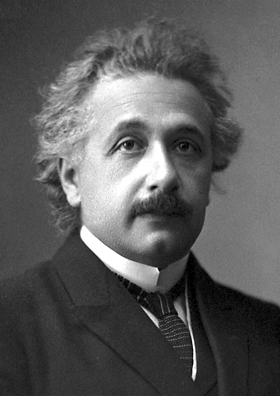
\includegraphics[height=6.8cm]{einstein_original_user.png}
  \caption{原图：皱纹、颗粒和局部明暗较明显}
\end{subfigure}
\hspace{0.06\textwidth}
\begin{subfigure}[t]{0.45\textwidth}
  \centering
  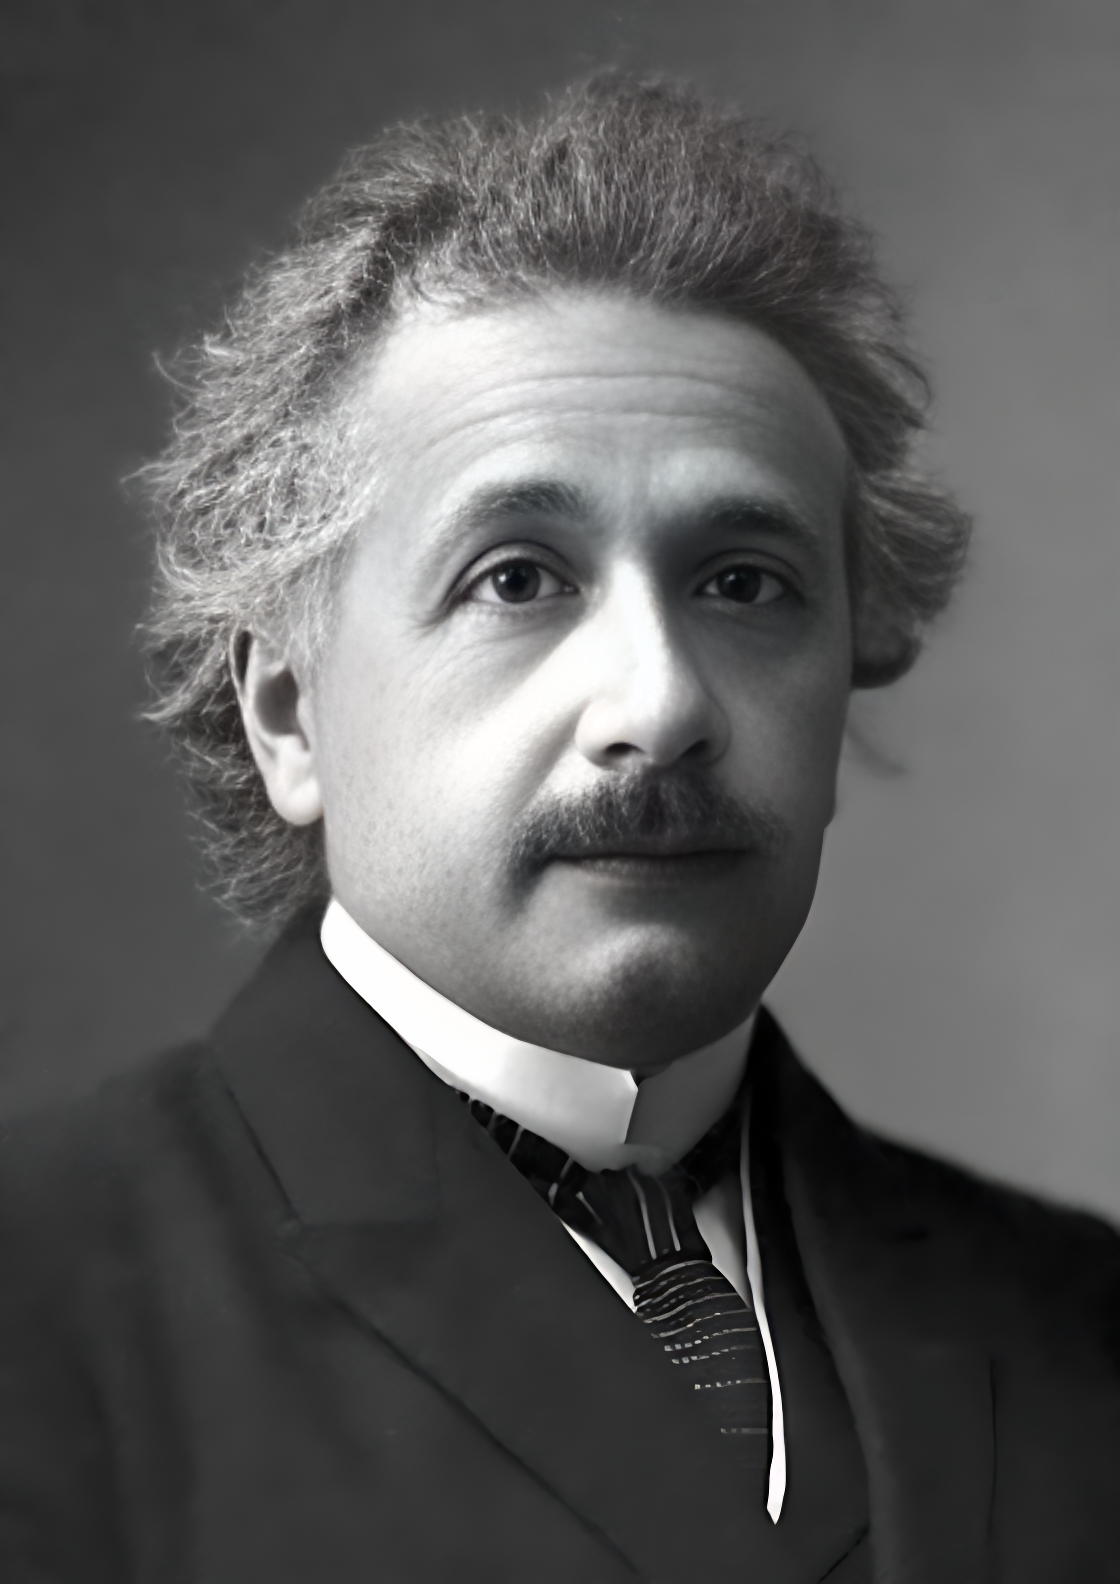
\includegraphics[height=6.8cm]{einstein_restored_user.png}
  \caption{修复图：噪声减少，但部分纹理被平滑或重绘}
\end{subfigure}
\caption{生成式修复同时带来去噪和纹理改写。该图用于说明现象，不作为定量实验结果。}
\label{fig:einstein}
\end{figure}

\section{CR-FIQA不能保证身份保持}

CR-FIQA用于预测一张人脸是否适合交给识别模型\cite{crfiqa}。我原本计划根据FIQA分数区分clear、marginal和poor，再决定是否建库、识别或超分。

我使用MEVID训练身份做过一次诊断。候选数据包含632条轨迹，其中118条得到有效人脸，最终形成39条参考记录和49条独立测试记录。

\begin{table}[H]
\centering
\caption{CR-FIQA在MEVID单帧协议中的诊断结果}
\label{tab:fiqa}
\begin{tabular}{lr}
\toprule
项目 & 结果\\
\midrule
ArcFace第一名正确 & 9/49（18.4\%）\\
第一名正确且达到0.45阈值 & 0/49\\
FIQA分数与是否认对的相关系数 & 0.026\\
不筛选时的第一名正确率 & 18.4\%\\
过滤最低10\% FIQA后 & 20.0\%\\
过滤最低20\% FIQA后 & 17.5\%\\
过滤最低50\% FIQA后 & 16.0\%\\
\bottomrule
\end{tabular}
\end{table}

FIQA高分人脸没有表现出更稳定的ArcFace识别结果。过滤最低10\%只产生轻微波动，继续过滤后识别率反而下降。因此，CR-FIQA不适合作为当前MEVID身份识别链路的单一决策依据。

正式GFPGAN实验进一步验证了这一点：156条配对样本的CR-FIQA原始分数从平均1.003上升到1.486，平均增加0.483；但ArcFace Rank-1明显下降，修复前后embedding平均余弦仅为0.402。CR-FIQA衡量识别可用性，但它不能证明生成式修复保留了同一身份。因此，本报告仅把FIQA作为诊断变量；在完成独立训练集与客户域校准前，FIQA不改变质量分桶、超分路由或C组成员，也不能把``FIQA上升''解释为``身份信息改善''。

\section{正式实验设计}

\subsection{固定Check-in Gallery与Query}

实验使用MEVID actor check-in正面照作为唯一人脸Gallery，不使用官方person ReID Gallery。Check-in压缩包含2,898张图片和172个数字前缀，覆盖全部104个train PID、54个test PID以及52个官方Query PID。官方资料没有单独发布映射表，因此实验同时保存编号覆盖审计与ArcFace sanity check，避免仅凭文件名假设映射。

Gallery只接收原始图中\texttt{direct + clear + can\_enroll=true}的人脸。最终选择343张check-in人脸，形成145个身份模板。52个Query PID中，0206和0294没有通过产品建库门控的check-in模板；结果保留这些Query并明确标记模板不可用，而不是静默删除。

316条官方Query轨迹均被纳入固定manifest。每条轨迹确定性均匀抽取24帧，用便宜的人体上部ROI代理维护Top-3候选，并加入body-best兜底；之后仅在候选上运行人脸检测和质量评估，使用产品共享的\texttt{face\_evidence\_rank}选择唯一face-best。选帧不读取身份预测结果。最终得到34条direct、40条recoverable、82条unusable和160条none。

\subsection{单轴质量分桶与双轴产品路由}

实验准备阶段考虑过两种设计。第一种设计只保留clear、marginal、poor和none质量类别，再把类别直接映射为原图识别、超分或拒绝。第二种设计同时输出质量类别和direct、recoverable、unusable、none可用状态。本实验采用第二种设计。这里的``双轴''不是运行两套互不相关的质量模型：两轴共享尺寸、检测置信度、姿态和模糊度等底层观测，但分别回答``图像质量如何''和``产品应采取什么动作''。

\begin{table}[H]
\centering
\caption{单轴质量类别驱动与双轴质量--可用状态设计对比}
\label{tab:quality-routing}
\renewcommand{\arraystretch}{1.18}
\begin{tabular}{p{0.17\textwidth}p{0.35\textwidth}p{0.38\textwidth}}
\toprule
设计 & 决策方式 & 优点与局限\\
\midrule
单轴类别驱动 &
先分为clear、marginal、poor和none，再为每个类别固定一种产品动作。 &
字段少、解释简单；但poor同时包含25像素可恢复小脸和8像素不可恢复小脸，marginal也可能同时包含可直接识别与值得尝试增强的样本。类别阈值变化会连带改变产品动作。\\
\addlinespace
双轴设计（采用） &
质量类别描述严重程度；可用状态根据缺陷类型和技术下限独立给出direct、recoverable、unusable或none。 &
能够区分``质量差但可处理''与``质量差且不可恢复''，便于安全拒绝、配置审计和冻结实验；代价是必须在文档和消费方中保持两类字段语义一致。\\
\bottomrule
\end{tabular}
\end{table}

具体而言，未检测到可用人脸时记为none；检测分数低于0.5、极端姿态，或人脸短边低于20像素时记为unusable。通过这些硬门槛后，短边位于20--28像素，或模糊程度落入配置化可恢复区间的人脸记为recoverable；其余可直接使用原图的人脸记为direct。质量类别不直接决定动作：一个poor样本可能因25像素小脸而recoverable，也可能因8像素小脸而unusable；一个marginal样本也可能保持direct。

冻结manifest生成时，156条可对齐Query均保存了CR-FIQA分数，但40条recoverable全部由20--28像素尺寸规则确定。反事实关闭FIQA后，这40条的成员完全不变；其中5条同时带有low-FIQA诊断标签，但该标签不是入组原因。因此，后续多超分后端实验继续复用相同manifest和eligibility，不重新分桶；超分前后FIQA只作为诊断统计，不参与C组路由或恢复后验收。

\subsection{三组固定处理}

三组共享同一check-in Gallery、Query face-best、ArcFace和0.45接受阈值：

\begin{table}[H]
\centering
\caption{A/B/C固定处理协议}
\label{tab:protocol}
\renewcommand{\arraystretch}{1.2}
\begin{tabular}{p{0.20\textwidth}p{0.70\textwidth}}
\toprule
组别 & 处理方式\\
\midrule
A：原图 & 所有已检测并对齐的face-best直接进入ArcFace；这是诊断对照，不代表产品会接受unusable样本。\\
B：全量超分 & 所有已检测并对齐的face-best先经过确定性GFPGAN，再进入ArcFace；GFPGAN失败时不回退A。\\
C：产品路由 & 不重新运行GFPGAN：direct读取缓存A，recoverable读取对应的缓存B，unusable和none不产生人脸向量；FIQA不改变该路由。\\
\bottomrule
\end{tabular}
\end{table}

所有输入、配置、模型权重和结果均保存SHA256。B组保存156张原始对齐脸、156张GFPGAN脸、embedding缓存以及156张完整对比图；C组只从缓存派生，不根据识别是否改善选择A或B。

\section{正式实验结果}

\subsection{总体与分组结果}

\begin{table}[H]
\centering
\caption{按产品eligibility分组的Rank-1结果。C在unusable和none上为0是主动拒绝，不是模型预测错误。}
\label{tab:formal-rank1}
\renewcommand{\arraystretch}{1.15}
\begin{tabular}{lrrrr}
\toprule
Query组 & 样本数 & A原图 & B全量GFPGAN & C产品门控\\
\midrule
全部官方Query & 316 & 25.3\% & 14.6\% & 11.7\%\\
\textbf{产品可用（direct+recoverable）} & \textbf{74} & \textbf{74.3\%} & \textbf{44.6\%} & \textbf{50.0\%}\\
direct & 34 & 85.3\% & 73.5\% & 85.3\%\\
recoverable & 40 & 65.0\% & 20.0\% & 20.0\%\\
unusable & 82 & 30.5\% & 15.9\% & 0.0\%\\
none & 160 & 0.0\% & 0.0\% & 0.0\%\\
\bottomrule
\end{tabular}
\end{table}

全量百分比包含160条none以及C主动拒绝的82条unusable，因此不能只用全量Rank-1评价产品门控。在74条产品可用Query中，C为37/74（50.0\%），高于B的33/74（44.6\%）：C保留34条direct原图，使该组从B的25/34恢复到29/34；40条recoverable仍使用缓存B，因此B和C同为8/40。C在全量统计中反而低于B，是因为它主动拒绝82条unusable，而B仍强制预测并碰巧认对13条。产品门控追求的是安全拒绝，不应把这些不可靠预测当作可部署收益。在固定0.45阈值下，产品可用组中C正确接受19条、B仅4条；两者的错误接受分别为1条和0条，但这里没有独立impostor cohort，不能称为正式FMR。

\subsection{Recoverable组的配对结果}

Recoverable组中，A组26/40第一名正确，B组仅8/40正确。配对转换如下：

\begin{table}[H]
\centering
\caption{Recoverable组A$\rightarrow$B的配对转换}
\label{tab:paired}
\begin{tabular}{lr}
\toprule
转换 & 数量\\
\midrule
原图错误，GFPGAN后正确 & 0\\
原图正确，GFPGAN后错误 & 18\\
两者都正确 & 8\\
两者都错误 & 14\\
\midrule
Rank-1净变化 & $-45$个百分点\\
95\% bootstrap置信区间 & $[-60,-30]$个百分点\\
精确配对双侧检验 & $p=7.63\times10^{-6}$\\
\bottomrule
\end{tabular}
\end{table}

结果不是由少量极端样本造成：置信区间整体低于0，且没有任何recoverable样本由错变对。Direct组也从29/34降到25/34；Unusable组从25/82降到13/82。这些结果一致指向身份信息损失。

\subsection{不同质量层级的审计图}

冻结数据中的category与eligibility并非同义词：9条clear和25条marginal均为direct，40条recoverable全部为poor，另有82条poor为unusable。图\ref{fig:quality-strata}分别从clear/direct、marginal/direct和poor/recoverable组中选择\texttt{rule\_quality}最接近组内中位数的样本，选择规则不读取A/B/C识别结果。

\begin{figure}[H]
\centering
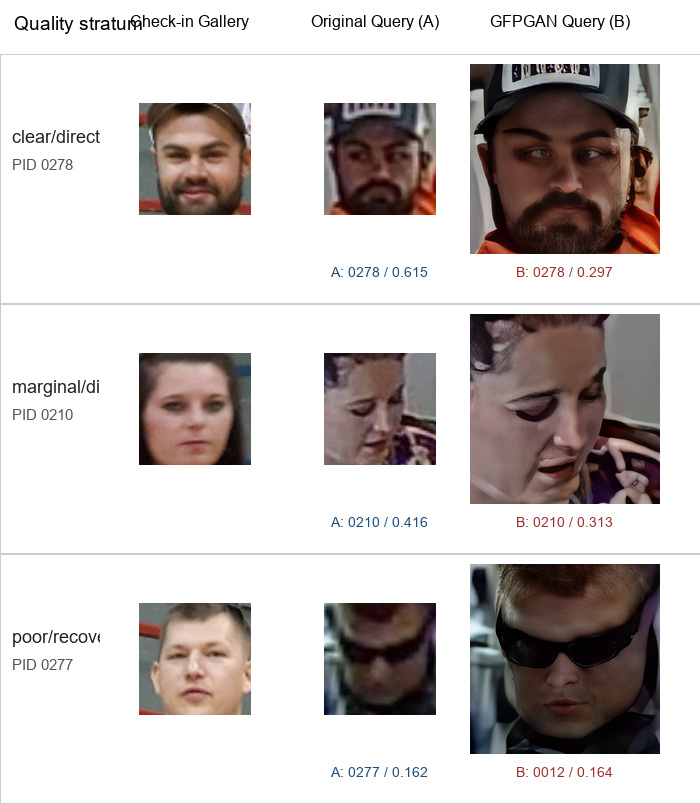
\includegraphics[height=0.73\textheight]{formal_quality_strata_grid.jpg}
\caption{按质量层级固定选择的三组Gallery--原始Query--GFPGAN Query审计图。三行依次为clear/direct（组内$n=9$）、marginal/direct（$n=25$）和poor/recoverable（$n=40$）。Clear样本的A/B分数为0.615/0.297，marginal样本为0.416/0.313；poor/recoverable样本从A正确识别0277（0.162）变为B错误识别0012（0.164）。每组均按\texttt{rule\_quality}中位数选择，视觉展示不参与样本选择和定量统计。}
\label{fig:quality-strata}
\end{figure}

\begin{figure}[H]
\centering
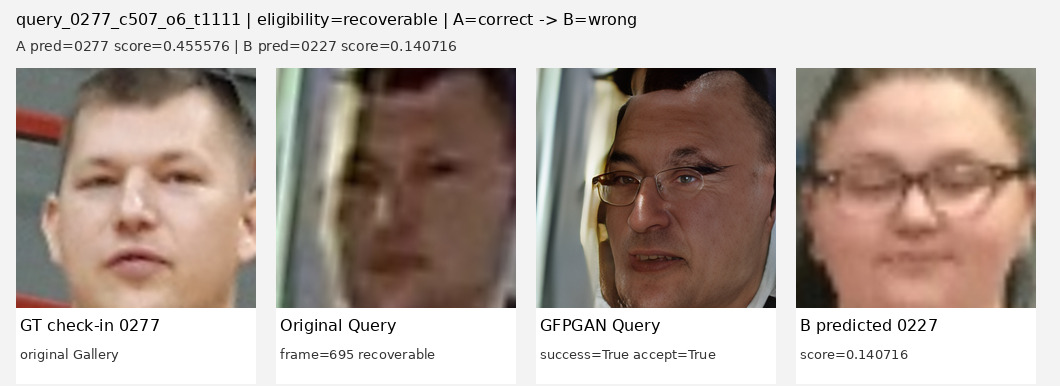
\includegraphics[width=\textwidth]{formal_recoverable_degradation.jpg}
\caption{预先定义的recoverable退化案例：在A正确、B错误的样本中，选择A分数最高的一条作审计展示。左起包含真实check-in Gallery、原始Query、GFPGAN Query及错误预测Gallery。原图对身份0277的第一名分数为0.46；GFPGAN后第一名变为0227，分数0.14。该图仅作单例解释，定量结论来自全部40条配对Query。}
\label{fig:formal-degradation}
\end{figure}

\subsection{视觉质量上升但身份特征漂移}

GFPGAN在Tesla T4上处理156张对齐脸，156次均产生图像并成功提取embedding。纯增强总耗时14.80秒，平均94.9毫秒/脸，不含模型首次启动。CR-FIQA原始分数平均增加0.483，但修复前后ArcFace embedding平均余弦只有0.402（中位数0.373）。因此，GFPGAN的主要问题不是运行失败或速度，而是它生成了更符合人脸先验、却偏离原身份特征的纹理。

全部156条B样本均保存真实check-in Gallery、原始Query、GFPGAN Query和必要的错误预测Gallery；没有只展示有利或不利案例。完整结果位于\path{/results/checkin_superres_abc_v3}，并已下载校验到本地结果目录。

\section{限制}

\begin{enumerate}[leftmargin=2.2em]
  \item MEVID提供裁剪后的人体轨迹，本实验不能评价全帧人物检测、track ID switch或脸体关联精度；
  \item Check-in编号完整覆盖MEVID身份，且ArcFace sanity check支持对应关系，但官方没有单独发布actor-to-PID映射表；
  \item 52个Query PID中有两个没有合格的check-in模板；实验没有独立impostor Query，因此``错误接受''不能称为正式FMR；
  \item 结论针对GFPGAN V1.3、ArcFace和当前MEVID监控条件，不能推广为GFPGAN对所有画面修复任务都无效。
\end{enumerate}

\section{产品建议}

现阶段，我建议：

\begin{enumerate}[leftmargin=2.2em]
  \item 身份识别默认关闭GFPGAN，direct人脸继续使用原始对齐脸；
  \item 当前recoverable状态表示输入满足技术处理下限，不表示GFPGAN能恢复身份；在获得新的正向证据前，该状态不应自动进入GFPGAN身份分支；
  \item 前端可以保留GFPGAN画面增强，明确标记为生成式修复结果；
  \item CR-FIQA保留为诊断信号；在独立校准证明其有效前，不用于改变质量分桶、超分路由或恢复后验收；
  \item 后续优先改进人脸感知选帧和多帧特征聚合，再评估专门以身份保持为目标训练的超分方法。
\end{enumerate}

\footnotesize
\begin{thebibliography}{9}

\bibitem{gfpgan}
X. Wang, Y. Li, H. Zhang, and Y. Shan,
``Towards Real-World Blind Face Restoration with Generative Facial Prior,''
\textit{Proceedings of the IEEE/CVF Conference on Computer Vision and Pattern Recognition},
2021.

\bibitem{perceptiondistortion}
Y. Blau and T. Michaeli,
``The Perception-Distortion Tradeoff,''
\textit{Proceedings of the IEEE/CVF Conference on Computer Vision and Pattern Recognition},
2018.

\bibitem{pulse}
S. Menon, A. Damian, S. Hu, N. Ravi, and C. Rudin,
``PULSE: Self-Supervised Photo Upsampling via Latent Space Exploration of Generative Models,''
\textit{Proceedings of the IEEE/CVF Conference on Computer Vision and Pattern Recognition},
2020.

\bibitem{crfiqa}
F. Boutros, M. Fang, M. Klemt, B. Fu, and N. Damer,
``CR-FIQA: Face Image Quality Assessment by Learning Sample Relative Classifiability,''
\textit{Proceedings of the IEEE/CVF Conference on Computer Vision and Pattern Recognition},
2023.

\end{thebibliography}
\normalsize

\end{document}
